%\section{Introduction}

\cs{T}his chapter describes the design, implementation, and evaluation of
\textbf{\rccns},
the router configuration checker, a tool
that uses static analysis to detect faults in Border Gateway Protocol
(BGP) 
configuration.  
By finding faults over a
distributed set of router configurations, \rcc enables network
operators to test and debug configurations before deploying them in an
operational network. This approach improves on the status quo of
``stimulus-response'' debugging where operators need to run
configurations in an operational network before finding faults.

As described in Chapter~\ref{chap:related} (Section~\ref{sec:conf}),
network operators use router configurations to provide reachability,
express routing policy (\eg, transit and peering
relationships~\cite{Norton2000}, inbound and outbound
routes~\cite{Beijnum2002}, etc.), configure primary and backup
links~\cite{Gao2001b}, and perform traffic engineering across multiple
links~\cite{Feamster2004}.  The complex process of configuring routers
is exacerbated by the number of lines of code, by configuration being
distributed across the routers in the network, by the absence of useful
high-level primitives in today's configuration languages, by the
diversity in vendor-specific configuration languages, and by the number
of ways in which the same high-level functionality can be expressed in a
configuration language.  

Router configuration gives network operators the flexibility to control
traffic and implement complex business relationships, but its complexity
also means that router configurations are prone to
faults~\cite{Beijnum2002,Mahajan2002}.  Configuration faults include
invalid routes (including hijacked and leaked routes); contract
violations~\cite{Feamster2004b}; unstable routes~\cite{labovitz:ton01};
routing loops~\cite{Dube99,Feamster2003b}; and persistently oscillating
routes~\cite{Basu2002,Griffin99,Varadhan2000}.
%Section~\ref{s:nanogproblems} discusses the problems observed in
%operational networks in detail.  
As summarized in
Table~\ref{tab:empirical_results} (Section~\ref{sec:rcc_related}), BGP
configuration faults can seriously affect end-to-end Internet
connectivity, leading to lost packets, forwarding loops, and unintended
paths between hosts or ASes.  


\begin{figure}[t]
\begin{center}
%\resizebox{0.8\columnwidth}{!}{\includegraphics*[viewport=100 200 500 650]{rcc/figures/nanog_table.pdf}}
\centering\epsfig{file=rcc/figures/nanog_table.eps, angle=270, width=\linewidth}
\end{center}
\caption{Number of threads discussing routing
  faults on the NANOG mailing list.
}
\label{tab:nanogerrors}
\end{figure}


%% Chapter~\ref{chap:related} (Section~\ref{sec:configuration})
%% describes how BGP's configuration affects which routes are originated
%% and propagated, how routes are modified as they propagate, which route
%% each router selects from multiple options, and how routes propagate
%% between routers.  
To understand the extent to which this complex configuration is
responsible for the types of failures that occur in practice, we studied
the archives of the North American Network Operators Group (NANOG)
mailing list, where network operators report operational problems,
discuss operational issues, etc.~\cite{nanog-list}.  Because the list
has received about 75,000 emails over the course of ten years, we first
clustered the emails by thread and pruned threads based on a list of
about fifteen keywords (\eg, ``BGP'', ``issue'', ``loop'', ``problem'',
``outage'').  We then reviewed these threads and classified each of them
into one or more of the categories shown in
Figure~\ref{tab:nanogerrors}.  This informal study shows some clear
trends.  First, many routing problems are caused by configuration
faults.  Second, the same types of problems continually appear.  Third,
BGP configuration problems continually perplex even experienced network
operators.  A tool like \rcc that can {\em proactively} detect
configuration faults will 
clearly benefit network operators.



Remarkably, static configuration analysis
can detect many of these configuration faults before the faulty
configuration is ever deployed on a live network.

Detecting BGP configuration faults poses several challenges beyond
simply defining a correctness specification.
%
First, a high-level correctness specification, such as the one defined
in Chapter~\ref{chap:rlogic}, must be used to derive a set of
constraints that can be tested against the actual configuration.
%
Second, BGP configuration is distributed---analyzing routing
configuration requires both synthesizing distributed configuration
fragments and representing the configuration in a form that makes it
easy to test constraints.
%
This chapter tackles these challenges and makes the following
two contributions:


\begin{enumerate}
\itemsep=-1pt
\item We present the design and implementation of {\bf \rccns}.
\rcc focuses on detecting faults that have the potential to cause {\em
  persistent} routing failures.  \rcc is not concerned with
correctness during convergence (since any distributed protocol will
have transient inconsistencies during convergence).  \rccns's goal is
to detect problems that may exist in the steady state, even when the
protocol converges to some stable outcome.

\item We use \rcc to explore the extent of real-world BGP
configuration faults; this chapter presents the first published analysis
of BGP configuration faults in real-world ISPs.  
We have analyzed real-world,
deployed configurations from 17 different ASes and detected more than
1,000 BGP configuration faults that had previously gone undetected by
operators.  These faults ranged from simple ``single router'' faults
(\eg, undefined variables) to complex, {\em network-wide} faults
involving interactions between multiple routers.  
To date, \rcc has been downloaded by over seventy network operators.
\end{enumerate}

\rcc is intended to be used {\em before} configurations are
deployed, but we also used \rcc to study the deployed configurations of live,
operational networks.  In these networks, \rcc discovered many
faults that could potentially cause failures.  These include: (1) faults
that could have caused network partitions due to errors in how external
BGP information was being propagated to routers inside an AS, (2) faults
that caused invalid routes to propagate inside an AS, and (3) faults in
policy expression that caused routers to advertise routes (and hence
potentially forward packets) in a manner inconsistent with the AS's
desired policies.
%
Our findings indicate that configuration faults that can
cause serious failures are often not immediately apparent (\ie, the
failure that results 
from a configuration fault may only be triggered by a specific failure
scenario or sequence of route advertisements).  If \rcc were used before
BGP configuration was deployed, we expect that it would be able to
detect faults that immediately caused routing failures as well.

Our analysis of real-world configurations suggests that most
configuration faults stem from three main causes.  First, the mechanisms
for propagating routes within a network are overly complex.  The main
techniques used to propagate routes scalably within a network (\eg,
``route reflection with clusters'') are easily misconfigured.  Second,
many configuration faults arise because configuration is distributed
across routers: even simple policy specifications require configuration
fragments on multiple routers in a network.  Third, configuring policy
often involves low-level mechanisms (\eg, ``route maps'', ``community
lists'', etc.)  that should be hidden from network operators.

The rest of this chapter proceeds as follows.
Section~\ref{sec:rcc_overview} describes the design of \rccns.
Sections~\ref{sec:visibility} and~\ref{sec:validity} highlight some of \rccns's
path visibility and route validity tests.
Section~\ref{sec:implementation} describes implementation details.
Section~\ref{sec:evaluation} presents configuration faults that \rcc
discovered in 17 operational networks.  Section~\ref{sec:rcc_lessons}
summarizes the take-away lessons from this study, and
Section~\ref{s:rcc_concl} concludes.
